\clearpage
\section{Closure Test for Template Method}
\label{sec:templateclosure}

The $E^{miss}_T$ template method is applied to MC to test its effectiveness under ‘ideal’ conditions. We construct
templates in MC using the procedure described in Sec.~\ref{sec:bkg_zjets}. The MC samples used for the construction of templates as well
as the sample used for $E^{miss}_T$  predictions is listed below. After these templates are constructed from the photon samples, 
they are then used to predict the $E^{miss}_T$ distribution in \zjets MC. The datasets used for the closure test are listed in table~\ref{tab:closuremc}

\begin{table}[htb]                                                                                                                                                              
\begin{center}                                                                                                                                                
\scriptsize
\caption{\label{tab:closuremc} List of MC samples used for the closure test.}
\begin{tabular}{l|l|c}  
\hline
\hline
Process & Dataset Name & Cross Section [pb] \\
\hline
$\gamma$ + Jets & \verb=/G_Pt-15to30_TuneZ2star_8TeV_pythia6/Summer12_DR53X-PU_S10_START53_V7A-v1/AODSIM= & 200061.7 \\
 & \verb=/G_Pt-30to50_TuneZ2star_8TeV_pythia6/Summer12_DR53X-PU_S10_START53_V7A-v1/AODSIM= & 19931.62 \\
 & \verb=/G_Pt-50to80_TuneZ2star_8TeV_pythia6/Summer12_DR53X-PU_S10_START53_V7A-v1/AODSIM= & 3322.309 \\
 & \verb=/G_Pt-80to120_TuneZ2star_8TeV_pythia6/Summer12_DR53X-PU_S10_START53_V7A-v1/AODSIM= & 558.2865 \\
 & \verb=/G_Pt-120to170_TuneZ2star_8TeV_pythia6/Summer12_DR53X-PU_S10_START53_V7A-v1/AODSIM= & 108.0068 \\
 & \verb=/G_Pt-170to300_TuneZ2star_8TeV_pythia6/Summer12_DR53X-PU_S10_START53_V7A-v1/AODSIM= & 30.12207 \\
 & \verb=/G_Pt-300to470_TuneZ2star_8TeV_pythia6/Summer12_DR53X-PU_S10_START53_V7A-v1/AODSIM= & 2.138632 \\
 & \verb=/G_Pt-470to800_TuneZ2star_8TeV_pythia6/Summer12_DR53X-PU_S10_START53_V7A-v1/AODSIM= & 0.2119244 \\
 & \verb=/G_Pt-800to1400_TuneZ2star_8TeV_pythia6/Summer12_DR53X-PU_S10_START53_V7A-v1/AODSIM= & 0.007077847 \\
\hline
$Z + Jets$ & \verb=/DYToEE_M-20_CT10_TuneZ2star_v2_8TeV-powheg-pythia6/Summer12_DR53X-PU_S10_START53_V7A-v1/AODSIM= & 1930.9940 \\
 & \verb=/DYToMuMu_M-20_CT10_TuneZ2star_v2_8TeV-powheg-pythia6/Summer12_DR53X-PU_S10_START53_V7A-v1/AODSIM= & 1930.9940 \\
\hline
\hline
\end{tabular}
\end{center}
\end{table}



\subsection{Selection}
\label{sec:closureselection}

The same preselection requirements from the section~\ref{sec:eventSelection}~are used to study the closure of the template method, specifically:

\begin{itemize}
\item Require two leptons (OS, SF) which both pass the lepton selection with \pt $>$ 20 \GeVc 
\item 81 GeV $<$ \mll $<$ 101 GeV
\item Require at least two jets both with \pt $> 30$ \GeVc~and $|\eta| < 2.5$ 
\end{itemize}

\subsection{Results}
\label{sec:closureresults}

The results of these tests are shown in Fig.~\ref{fig:inclusiveclosure}, and Fig.~\ref{fig:targetedclosure}. Additionally, the yields are listed
in table~\ref{table:inclusive}, and table~\ref{table:targeted}.
%% inclusive plot
\begin{figure}[!h]
\begin{center}
\begin{tabular}{cc}
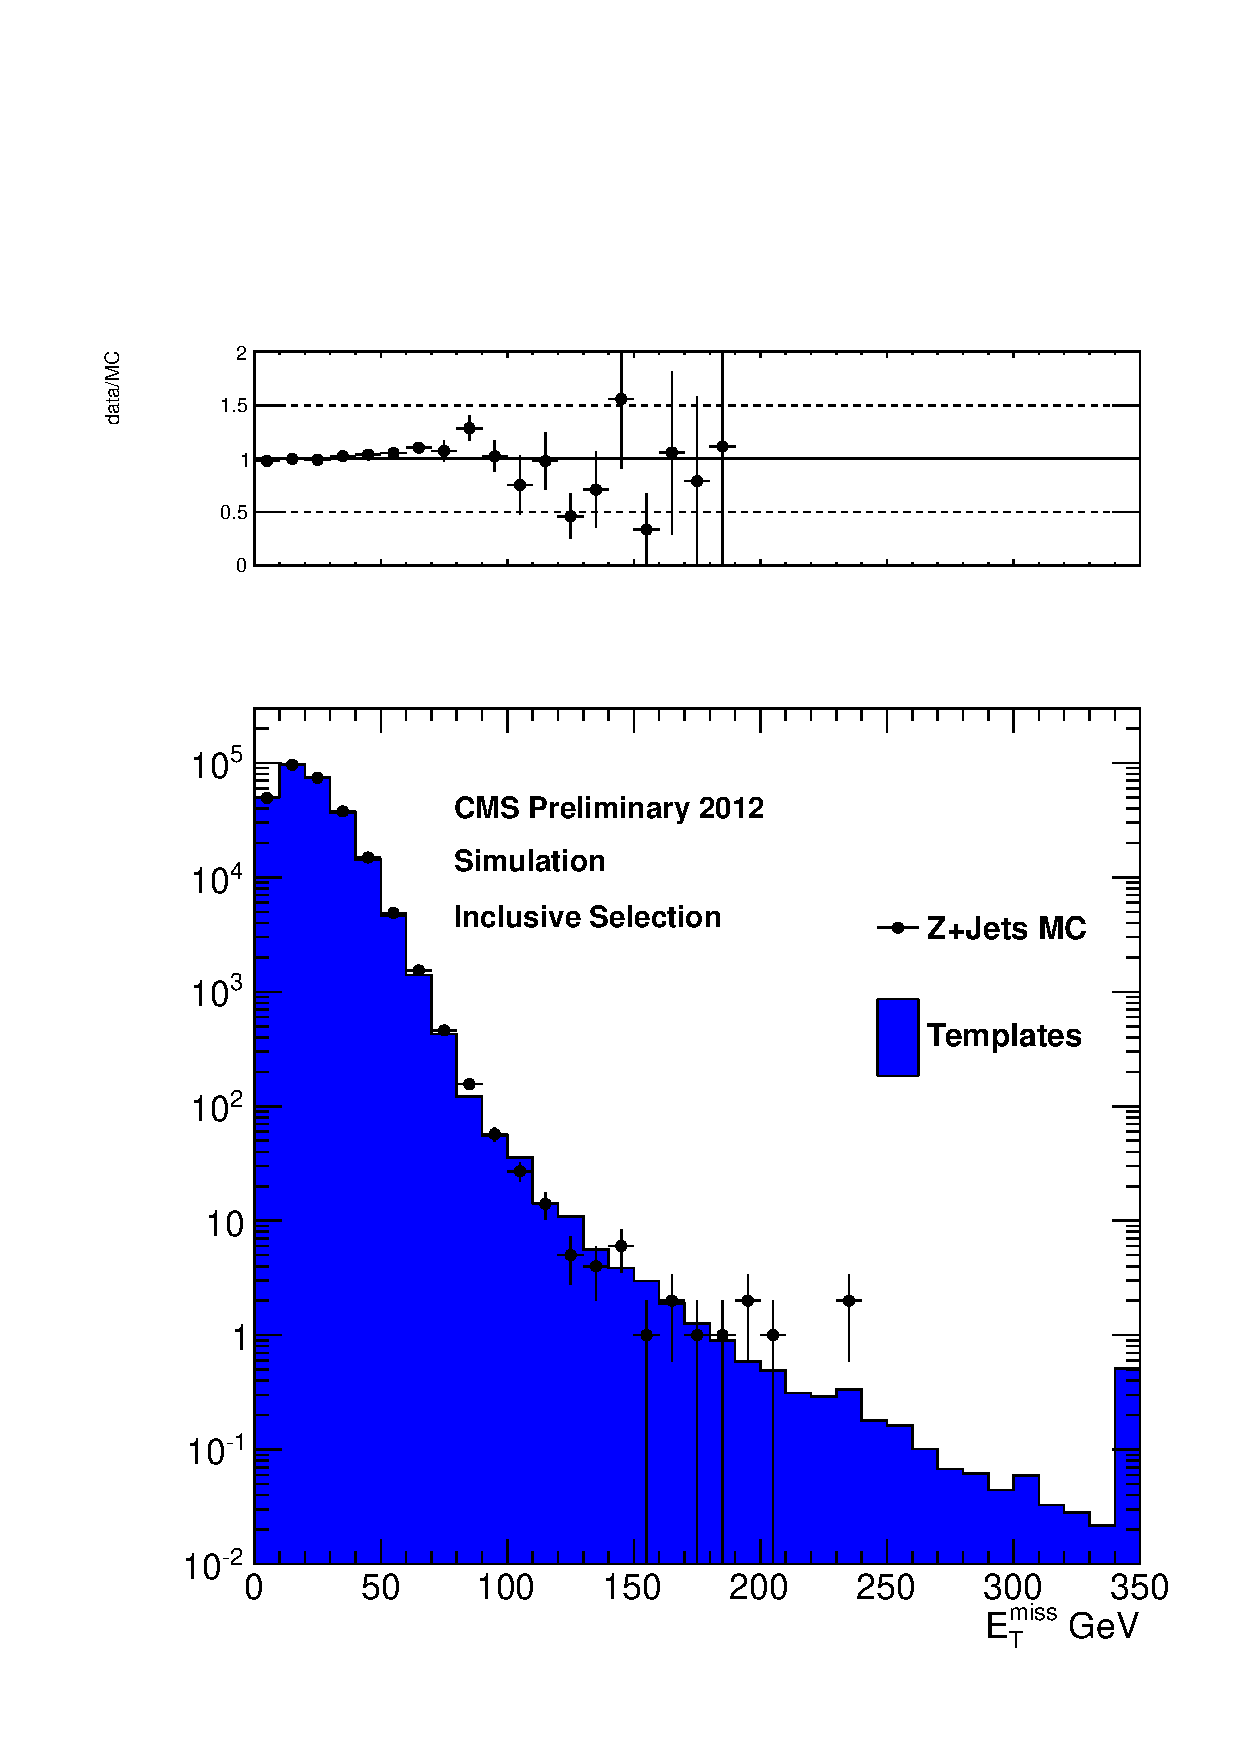
\includegraphics[width=0.6\textwidth]{plots/closure_inclusive.pdf}
\end{tabular}
\caption{The $E^{miss}_T$ distribution in $Z$ + jets MC (black) and prediction (blue) using the inclusive analysis selection. See Table~\ref{table:inclusive}~for integrals.
\label{fig:inclusiveclosure}
}
\end{center}
\end{figure}

\begin{table}[htb]
\scriptsize
\begin{center}
\caption{\label{table:inclusive} Results of MC closure tests for the inclusive analysis selections listed in section~\ref{sec:eventSelection}. The first row shows the yields from the $E^{miss}_T$ templates made from the photon sample. The second row shows the yield in DY MC. The third row shows the ratio of the DY Yield to the prediction from the templates.̄ All uncertainties shown are statistical only. }
\begin{tabular}{l|c|c|c|c|c|c}
\hline
\hline
          & $0 < \MET < 30$  & $30 < \MET < 60$  & $60 < \MET < 100$  & $100 < \MET < 200$  & $200 < \MET < 300$  &    $\MET > 300$  \\ 
\hline
DY Yields & 219941 $\pm$ 469.0 & 57483 $\pm$ 239.8 &  2212 $\pm$ 47.0 &     63 $\pm$ 7.9 &      3 $\pm$ 1.7 &      0 $\pm$ 1.0 \\
Templates & 221801.0 $\pm$ 943.7 & 55818.6 $\pm$ 493.2 & 2001.6 $\pm$ 66.4 & 78.1 $\pm$ 11.4 &   2.0 $\pm$ 0.18 &   0.7 $\pm$ 0.39 \\
    MC/BG & 99.2 $\pm$ 0.48 \% & 103.0 $\pm$ 0.98 \% & 110.5 $\pm$ 3.94 \% & 80.7 $\pm$ 19.24 \% & 146.6 $\pm$ 58.42 \% & 0.0 \% \\
\hline
\hline
\end{tabular}
\end{center}
\end{table}

%% targeted plot
\begin{figure}[!h]
\begin{center}
\begin{tabular}{cc}
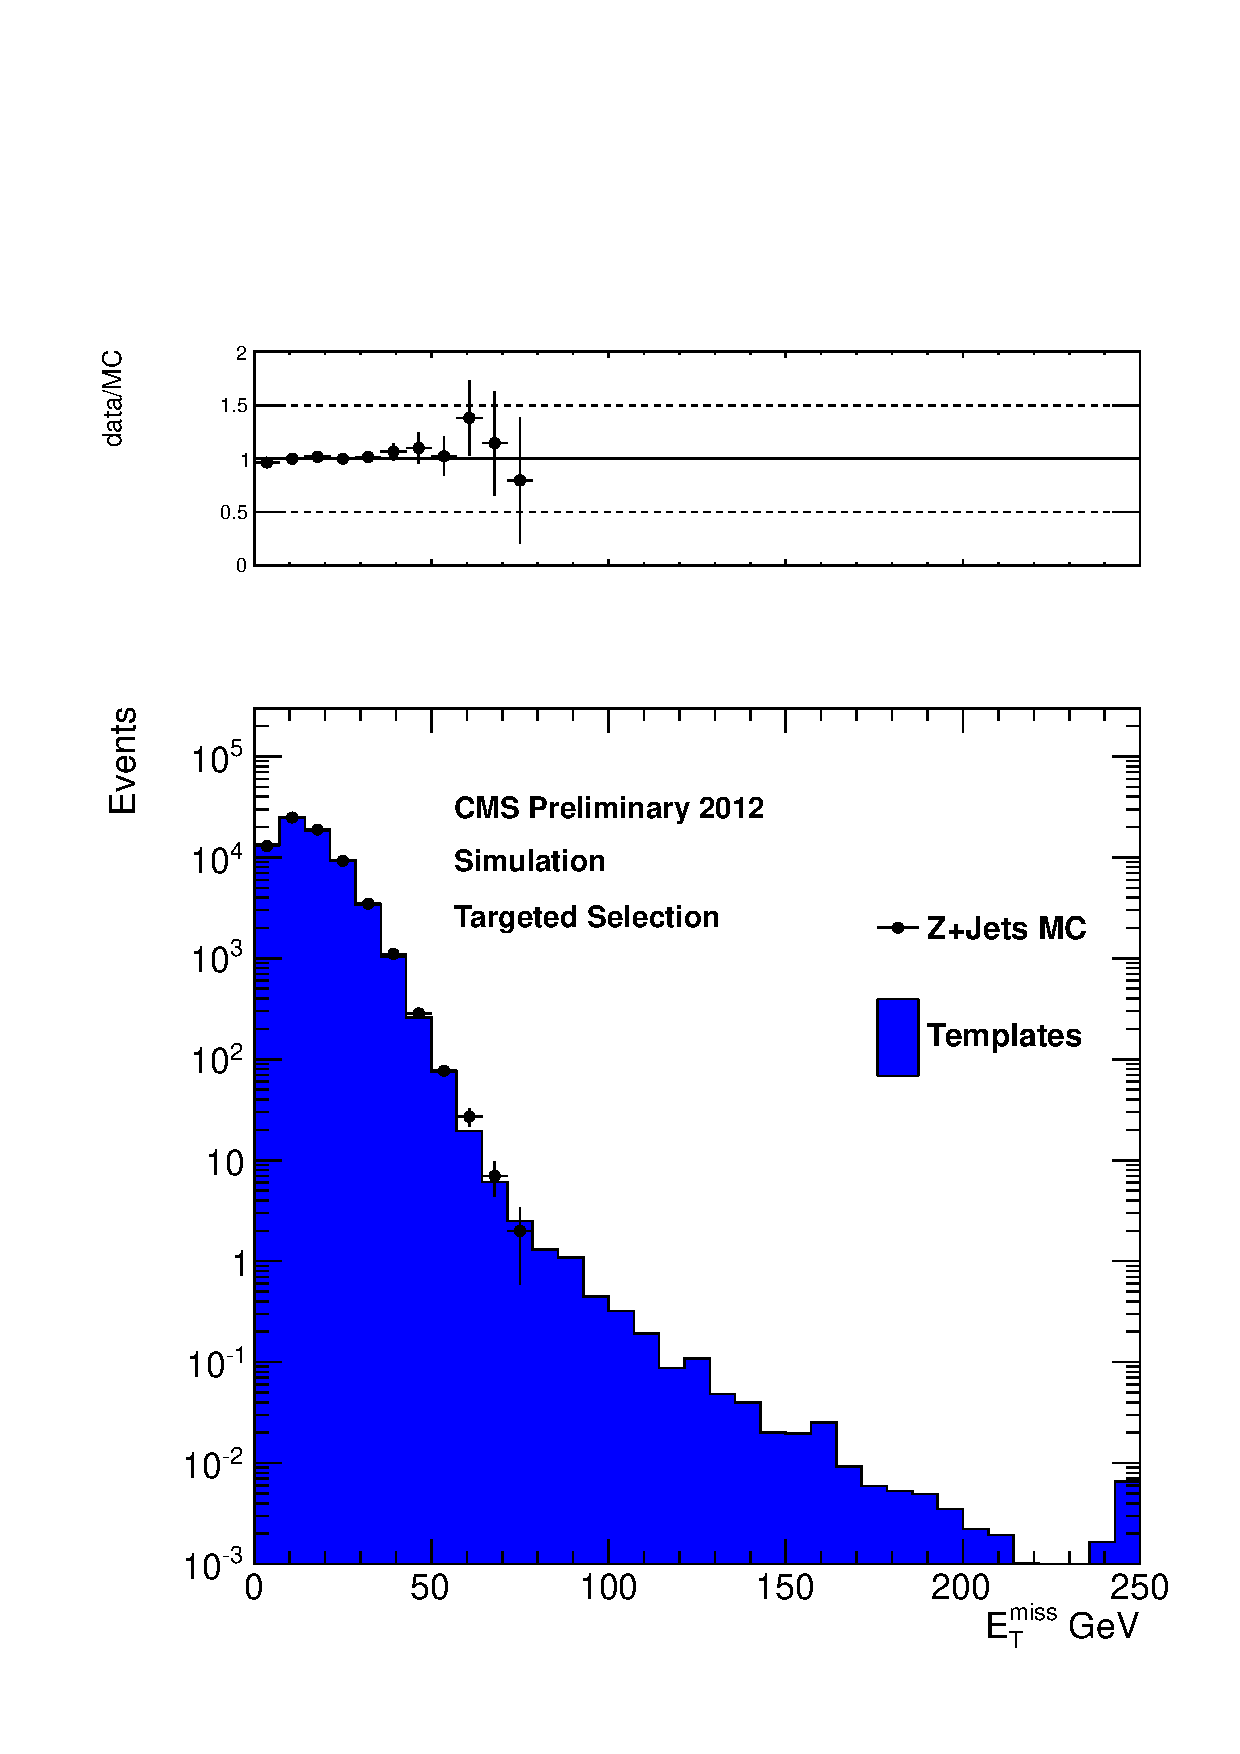
\includegraphics[width=0.6\textwidth]{plots/closure_targeted.pdf}
\end{tabular}
\caption{The $E^{miss}_T$ distribution in $Z$ + jets MC (black) and prediction (blue) using the targeted analysis selection. See Table~\ref{table:inclusive}~for integrals.
\label{fig:targetedclosure}
}
\end{center}
\end{figure}

\begin{table}[htb]
\scriptsize
\begin{center}
\caption{\label{table:targeted} Results of MC closure tests for the targeted analysis selections listed in section~\ref{sec:eventSelection}. The first row shows the yields from the $E^{miss}_T$ templates made from the photon sample. The second row shows the yield in DY MC. The third row shows the ratio of the DY Yield to the prediction from the templates.̄ All uncertainties shown are statistical only. }
\begin{tabular}{l|c|c|c|c}
\hline
\hline
          & $0 < \MET < 30$  & $30 < \MET < 60$  & $60 < \MET < 80$  & $80 < \MET < 100$  \\ 
\hline
DY Yields & 56620 $\pm$ 237.9 & 13843 $\pm$ 117.7 &   362 $\pm$ 19.0 &     34 $\pm$ 5.8 \\
Templates & 56769.0 $\pm$ 540.5 & 13725.9 $\pm$ 290.3 & 334.3 $\pm$ 31.7 &  25.7 $\pm$ 3.4 \\
    MC/BG & 99.7 $\pm$ 1.04 \% & 100.9 $\pm$ 2.28 \% & 108.3 $\pm$ 10.83 \% & 132.5 $\pm$ 21.65 \% \\
\hline
\hline
          & $100 < \MET < 120$  & $120 < \MET < 150$  & $150 < \MET < 200$  &    $200 < \MET$  \\ 
\hline
DY Yields &      2 $\pm$ 1.4 &      0 $\pm$ 1.0 &      0 $\pm$ 1.0 &      0 $\pm$ 1.0 \\
Templates &   3.8 $\pm$ 0.58 &   1.9 $\pm$ 0.24 &   0.5 $\pm$ 0.09 &   0.1 $\pm$ 0.02 \\
    MC/BG & 52.5 $\pm$ 72.34 \% & 0.0 \% & 0.0 \% & 0.0 \% \\
\hline
\hline
\end{tabular}
\end{center}
\end{table}

\clearpage
